% Options for packages loaded elsewhere
\PassOptionsToPackage{unicode}{hyperref}
\PassOptionsToPackage{hyphens}{url}
\PassOptionsToPackage{dvipsnames,svgnames,x11names}{xcolor}
%
\documentclass[
  letterpaper,
  DIV=11,
  numbers=noendperiod]{scrartcl}

\usepackage{amsmath,amssymb}
\usepackage{iftex}
\ifPDFTeX
  \usepackage[T1]{fontenc}
  \usepackage[utf8]{inputenc}
  \usepackage{textcomp} % provide euro and other symbols
\else % if luatex or xetex
  \usepackage{unicode-math}
  \defaultfontfeatures{Scale=MatchLowercase}
  \defaultfontfeatures[\rmfamily]{Ligatures=TeX,Scale=1}
\fi
\usepackage{lmodern}
\ifPDFTeX\else  
    % xetex/luatex font selection
\fi
% Use upquote if available, for straight quotes in verbatim environments
\IfFileExists{upquote.sty}{\usepackage{upquote}}{}
\IfFileExists{microtype.sty}{% use microtype if available
  \usepackage[]{microtype}
  \UseMicrotypeSet[protrusion]{basicmath} % disable protrusion for tt fonts
}{}
\makeatletter
\@ifundefined{KOMAClassName}{% if non-KOMA class
  \IfFileExists{parskip.sty}{%
    \usepackage{parskip}
  }{% else
    \setlength{\parindent}{0pt}
    \setlength{\parskip}{6pt plus 2pt minus 1pt}}
}{% if KOMA class
  \KOMAoptions{parskip=half}}
\makeatother
\usepackage{xcolor}
\setlength{\emergencystretch}{3em} % prevent overfull lines
\setcounter{secnumdepth}{-\maxdimen} % remove section numbering
% Make \paragraph and \subparagraph free-standing
\makeatletter
\ifx\paragraph\undefined\else
  \let\oldparagraph\paragraph
  \renewcommand{\paragraph}{
    \@ifstar
      \xxxParagraphStar
      \xxxParagraphNoStar
  }
  \newcommand{\xxxParagraphStar}[1]{\oldparagraph*{#1}\mbox{}}
  \newcommand{\xxxParagraphNoStar}[1]{\oldparagraph{#1}\mbox{}}
\fi
\ifx\subparagraph\undefined\else
  \let\oldsubparagraph\subparagraph
  \renewcommand{\subparagraph}{
    \@ifstar
      \xxxSubParagraphStar
      \xxxSubParagraphNoStar
  }
  \newcommand{\xxxSubParagraphStar}[1]{\oldsubparagraph*{#1}\mbox{}}
  \newcommand{\xxxSubParagraphNoStar}[1]{\oldsubparagraph{#1}\mbox{}}
\fi
\makeatother

\usepackage{color}
\usepackage{fancyvrb}
\newcommand{\VerbBar}{|}
\newcommand{\VERB}{\Verb[commandchars=\\\{\}]}
\DefineVerbatimEnvironment{Highlighting}{Verbatim}{commandchars=\\\{\}}
% Add ',fontsize=\small' for more characters per line
\usepackage{framed}
\definecolor{shadecolor}{RGB}{241,243,245}
\newenvironment{Shaded}{\begin{snugshade}}{\end{snugshade}}
\newcommand{\AlertTok}[1]{\textcolor[rgb]{0.68,0.00,0.00}{#1}}
\newcommand{\AnnotationTok}[1]{\textcolor[rgb]{0.37,0.37,0.37}{#1}}
\newcommand{\AttributeTok}[1]{\textcolor[rgb]{0.40,0.45,0.13}{#1}}
\newcommand{\BaseNTok}[1]{\textcolor[rgb]{0.68,0.00,0.00}{#1}}
\newcommand{\BuiltInTok}[1]{\textcolor[rgb]{0.00,0.23,0.31}{#1}}
\newcommand{\CharTok}[1]{\textcolor[rgb]{0.13,0.47,0.30}{#1}}
\newcommand{\CommentTok}[1]{\textcolor[rgb]{0.37,0.37,0.37}{#1}}
\newcommand{\CommentVarTok}[1]{\textcolor[rgb]{0.37,0.37,0.37}{\textit{#1}}}
\newcommand{\ConstantTok}[1]{\textcolor[rgb]{0.56,0.35,0.01}{#1}}
\newcommand{\ControlFlowTok}[1]{\textcolor[rgb]{0.00,0.23,0.31}{\textbf{#1}}}
\newcommand{\DataTypeTok}[1]{\textcolor[rgb]{0.68,0.00,0.00}{#1}}
\newcommand{\DecValTok}[1]{\textcolor[rgb]{0.68,0.00,0.00}{#1}}
\newcommand{\DocumentationTok}[1]{\textcolor[rgb]{0.37,0.37,0.37}{\textit{#1}}}
\newcommand{\ErrorTok}[1]{\textcolor[rgb]{0.68,0.00,0.00}{#1}}
\newcommand{\ExtensionTok}[1]{\textcolor[rgb]{0.00,0.23,0.31}{#1}}
\newcommand{\FloatTok}[1]{\textcolor[rgb]{0.68,0.00,0.00}{#1}}
\newcommand{\FunctionTok}[1]{\textcolor[rgb]{0.28,0.35,0.67}{#1}}
\newcommand{\ImportTok}[1]{\textcolor[rgb]{0.00,0.46,0.62}{#1}}
\newcommand{\InformationTok}[1]{\textcolor[rgb]{0.37,0.37,0.37}{#1}}
\newcommand{\KeywordTok}[1]{\textcolor[rgb]{0.00,0.23,0.31}{\textbf{#1}}}
\newcommand{\NormalTok}[1]{\textcolor[rgb]{0.00,0.23,0.31}{#1}}
\newcommand{\OperatorTok}[1]{\textcolor[rgb]{0.37,0.37,0.37}{#1}}
\newcommand{\OtherTok}[1]{\textcolor[rgb]{0.00,0.23,0.31}{#1}}
\newcommand{\PreprocessorTok}[1]{\textcolor[rgb]{0.68,0.00,0.00}{#1}}
\newcommand{\RegionMarkerTok}[1]{\textcolor[rgb]{0.00,0.23,0.31}{#1}}
\newcommand{\SpecialCharTok}[1]{\textcolor[rgb]{0.37,0.37,0.37}{#1}}
\newcommand{\SpecialStringTok}[1]{\textcolor[rgb]{0.13,0.47,0.30}{#1}}
\newcommand{\StringTok}[1]{\textcolor[rgb]{0.13,0.47,0.30}{#1}}
\newcommand{\VariableTok}[1]{\textcolor[rgb]{0.07,0.07,0.07}{#1}}
\newcommand{\VerbatimStringTok}[1]{\textcolor[rgb]{0.13,0.47,0.30}{#1}}
\newcommand{\WarningTok}[1]{\textcolor[rgb]{0.37,0.37,0.37}{\textit{#1}}}

\providecommand{\tightlist}{%
  \setlength{\itemsep}{0pt}\setlength{\parskip}{0pt}}\usepackage{longtable,booktabs,array}
\usepackage{calc} % for calculating minipage widths
% Correct order of tables after \paragraph or \subparagraph
\usepackage{etoolbox}
\makeatletter
\patchcmd\longtable{\par}{\if@noskipsec\mbox{}\fi\par}{}{}
\makeatother
% Allow footnotes in longtable head/foot
\IfFileExists{footnotehyper.sty}{\usepackage{footnotehyper}}{\usepackage{footnote}}
\makesavenoteenv{longtable}
\usepackage{graphicx}
\makeatletter
\def\maxwidth{\ifdim\Gin@nat@width>\linewidth\linewidth\else\Gin@nat@width\fi}
\def\maxheight{\ifdim\Gin@nat@height>\textheight\textheight\else\Gin@nat@height\fi}
\makeatother
% Scale images if necessary, so that they will not overflow the page
% margins by default, and it is still possible to overwrite the defaults
% using explicit options in \includegraphics[width, height, ...]{}
\setkeys{Gin}{width=\maxwidth,height=\maxheight,keepaspectratio}
% Set default figure placement to htbp
\makeatletter
\def\fps@figure{htbp}
\makeatother

\KOMAoption{captions}{tableheading}
\makeatletter
\@ifpackageloaded{caption}{}{\usepackage{caption}}
\AtBeginDocument{%
\ifdefined\contentsname
  \renewcommand*\contentsname{Table of contents}
\else
  \newcommand\contentsname{Table of contents}
\fi
\ifdefined\listfigurename
  \renewcommand*\listfigurename{List of Figures}
\else
  \newcommand\listfigurename{List of Figures}
\fi
\ifdefined\listtablename
  \renewcommand*\listtablename{List of Tables}
\else
  \newcommand\listtablename{List of Tables}
\fi
\ifdefined\figurename
  \renewcommand*\figurename{Figure}
\else
  \newcommand\figurename{Figure}
\fi
\ifdefined\tablename
  \renewcommand*\tablename{Table}
\else
  \newcommand\tablename{Table}
\fi
}
\@ifpackageloaded{float}{}{\usepackage{float}}
\floatstyle{ruled}
\@ifundefined{c@chapter}{\newfloat{codelisting}{h}{lop}}{\newfloat{codelisting}{h}{lop}[chapter]}
\floatname{codelisting}{Listing}
\newcommand*\listoflistings{\listof{codelisting}{List of Listings}}
\makeatother
\makeatletter
\makeatother
\makeatletter
\@ifpackageloaded{caption}{}{\usepackage{caption}}
\@ifpackageloaded{subcaption}{}{\usepackage{subcaption}}
\makeatother

\ifLuaTeX
  \usepackage{selnolig}  % disable illegal ligatures
\fi
\usepackage{bookmark}

\IfFileExists{xurl.sty}{\usepackage{xurl}}{} % add URL line breaks if available
\urlstyle{same} % disable monospaced font for URLs
\hypersetup{
  pdftitle={Check-in 1},
  colorlinks=true,
  linkcolor={blue},
  filecolor={Maroon},
  citecolor={Blue},
  urlcolor={Blue},
  pdfcreator={LaTeX via pandoc}}


\title{Check-in 1}
\author{}
\date{}

\begin{document}
\maketitle


\begin{Shaded}
\begin{Highlighting}[]
\FunctionTok{library}\NormalTok{(tidyverse)}
\end{Highlighting}
\end{Shaded}

\begin{verbatim}
-- Attaching core tidyverse packages ------------------------ tidyverse 2.0.0 --
v dplyr     1.1.4     v readr     2.1.5
v forcats   1.0.0     v stringr   1.5.1
v ggplot2   3.5.1     v tibble    3.2.1
v lubridate 1.9.3     v tidyr     1.3.1
v purrr     1.0.2     
-- Conflicts ------------------------------------------ tidyverse_conflicts() --
x dplyr::filter() masks stats::filter()
x dplyr::lag()    masks stats::lag()
i Use the conflicted package (<http://conflicted.r-lib.org/>) to force all conflicts to become errors
\end{verbatim}

\begin{Shaded}
\begin{Highlighting}[]
\FunctionTok{library}\NormalTok{(ggplot2)}
\FunctionTok{library}\NormalTok{(dplyr)}
\FunctionTok{library}\NormalTok{(janitor)}
\end{Highlighting}
\end{Shaded}

\begin{verbatim}

Attaching package: 'janitor'

The following objects are masked from 'package:stats':

    chisq.test, fisher.test
\end{verbatim}

\begin{Shaded}
\begin{Highlighting}[]
\FunctionTok{library}\NormalTok{(lubridate)}
\FunctionTok{library}\NormalTok{(here)}
\end{Highlighting}
\end{Shaded}

\begin{verbatim}
here() starts at C:/Users/aidan/OneDrive/Documents/GitHub/EPI-569-Final-Project
\end{verbatim}

\begin{Shaded}
\begin{Highlighting}[]
\NormalTok{ rff\_2024 }\OtherTok{\textless{}{-}} \FunctionTok{readRDS}\NormalTok{(}\FunctionTok{here}\NormalTok{(}\StringTok{"data/rff\_2024.rds"}\NormalTok{))}

\NormalTok{roster\_2024 }\OtherTok{\textless{}{-}} \FunctionTok{readRDS}\NormalTok{(}\FunctionTok{here}\NormalTok{(}\StringTok{"data/roster\_2024.rds"}\NormalTok{))}

\NormalTok{transmission\_pairs\_2024 }\OtherTok{\textless{}{-}} \FunctionTok{readRDS}\NormalTok{(}\FunctionTok{here}\NormalTok{(}\StringTok{"data/transmission\_pairs\_2024.rds"}\NormalTok{))}
\end{Highlighting}
\end{Shaded}

\begin{enumerate}
\def\labelenumi{\arabic{enumi}.}
\tightlist
\item
  Make a preliminary assessment of the data
\end{enumerate}

\begin{Shaded}
\begin{Highlighting}[]
\NormalTok{variables\_to\_check }\OtherTok{\textless{}{-}} \FunctionTok{c}\NormalTok{(}\StringTok{"Date\_of\_Onset"}\NormalTok{, }\StringTok{"Date\_of\_Recovery"}\NormalTok{)}

\NormalTok{missing\_counts }\OtherTok{\textless{}{-}} \FunctionTok{sapply}\NormalTok{(rff\_2024[variables\_to\_check], }\ControlFlowTok{function}\NormalTok{(x) }\FunctionTok{sum}\NormalTok{(}\FunctionTok{is.na}\NormalTok{(x)))}

\NormalTok{missing\_proportions }\OtherTok{\textless{}{-}} \FunctionTok{sapply}\NormalTok{(rff\_2024[variables\_to\_check], }\ControlFlowTok{function}\NormalTok{(x) }\FunctionTok{mean}\NormalTok{(}\FunctionTok{is.na}\NormalTok{(x)) }\SpecialCharTok{*} \DecValTok{100}\NormalTok{)}

\NormalTok{missing\_summary }\OtherTok{\textless{}{-}} \FunctionTok{data.frame}\NormalTok{(}
  \AttributeTok{Variable =}\NormalTok{ variables\_to\_check,}
  \AttributeTok{Missing\_Count =}\NormalTok{ missing\_counts,}
  \AttributeTok{Missing\_Percentage =}\NormalTok{ missing\_proportions}
\NormalTok{)}

\FunctionTok{print}\NormalTok{(missing\_summary)}
\end{Highlighting}
\end{Shaded}

\begin{verbatim}
                         Variable Missing_Count Missing_Percentage
Date_of_Onset       Date_of_Onset            35           38.46154
Date_of_Recovery Date_of_Recovery            35           38.46154
\end{verbatim}

\begin{enumerate}
\def\labelenumi{\alph{enumi}.}
\tightlist
\item
  What concerns do you have about the dataset?
\end{enumerate}

The dataset presents significant missing data issues, particularly when
reviewing the Date\_of\_Onset and Date\_of\_Recovery columns. Both
variables have 35 missing values, representing 38.46\% of the data in
each column. This high percentage of missing data could pose a
substantial challenge for any analysis that relies on the timing of
these events, such as understanding the progression of disease or
calculating time intervals between onset and recovery. The missing data
could introduce bias if some individuals were excluded from reporting or
if data collection needed to be more consistent across specific periods
or groups. If this missing data is addressed, it may maintain analysis,
particularly in modeling the duration of illness or treatment effects.

\begin{enumerate}
\def\labelenumi{\alph{enumi}.}
\setcounter{enumi}{1}
\tightlist
\item
  What cleaning or restructuring of the data may be required?
\end{enumerate}

Several cleaning and restructuring steps were performed based on the
analysis of missing data and potential issues in the dataset. The
significant missing values in the Date\_of\_Onset and Date\_of\_Recovery
variables (38.46\% missing in each) were addressed by removing
observations with missing values. As a result, out of the original 91
cases, only 56 remain for analysis. This reduction in sample size may
impact the generalizability of the findings and should be considered
when drawing conclusions from the analysis. Additionally, the dataset
was cleaned by ensuring consistency in date formats and verifying the
logical order of Date\_of\_Recovery relative to Date\_of\_Onset. These
steps improved the quality of the dataset, making it more suitable for
analysis.

\begin{enumerate}
\def\labelenumi{\arabic{enumi}.}
\setcounter{enumi}{1}
\tightlist
\item
  Epicurve and SIR plot
\end{enumerate}

\begin{Shaded}
\begin{Highlighting}[]
\FunctionTok{tabyl}\NormalTok{(rff\_2024}\SpecialCharTok{$}\StringTok{\textasciigrave{}}\AttributeTok{Date\_of\_Onset}\StringTok{\textasciigrave{}}\NormalTok{)}
\end{Highlighting}
\end{Shaded}

\begin{verbatim}
 rff_2024$Date_of_Onset  n    percent valid_percent
             2024-09-09  1 0.01098901    0.01785714
             2024-09-11  1 0.01098901    0.01785714
             2024-09-12  3 0.03296703    0.05357143
             2024-09-13  1 0.01098901    0.01785714
             2024-09-14  3 0.03296703    0.05357143
             2024-09-15  3 0.03296703    0.05357143
             2024-09-16  1 0.01098901    0.01785714
             2024-09-20  4 0.04395604    0.07142857
             2024-09-21  3 0.03296703    0.05357143
             2024-09-22  1 0.01098901    0.01785714
             2024-09-23  4 0.04395604    0.07142857
             2024-09-24  1 0.01098901    0.01785714
             2024-09-25  2 0.02197802    0.03571429
             2024-09-26  1 0.01098901    0.01785714
             2024-09-28  2 0.02197802    0.03571429
             2024-09-30  2 0.02197802    0.03571429
             2024-10-01  6 0.06593407    0.10714286
             2024-10-02  6 0.06593407    0.10714286
             2024-10-03  5 0.05494505    0.08928571
             2024-10-04  2 0.02197802    0.03571429
             2024-10-05  1 0.01098901    0.01785714
             2024-10-11  2 0.02197802    0.03571429
             2024-10-12  1 0.01098901    0.01785714
                   <NA> 35 0.38461538            NA
\end{verbatim}

\begin{Shaded}
\begin{Highlighting}[]
\FunctionTok{class}\NormalTok{(rff\_2024}\SpecialCharTok{$}\StringTok{\textasciigrave{}}\AttributeTok{Date\_of\_Onset}\StringTok{\textasciigrave{}}\NormalTok{)}
\end{Highlighting}
\end{Shaded}

\begin{verbatim}
[1] "Date"
\end{verbatim}

\begin{Shaded}
\begin{Highlighting}[]
\NormalTok{epicurveonset }\OtherTok{\textless{}{-}}\NormalTok{rff\_2024 }\SpecialCharTok{\%\textgreater{}\%}
    \FunctionTok{filter}\NormalTok{(}\SpecialCharTok{!}\FunctionTok{is.na}\NormalTok{(}\StringTok{\textasciigrave{}}\AttributeTok{Date\_of\_Onset}\StringTok{\textasciigrave{}}\NormalTok{)) }\SpecialCharTok{\%\textgreater{}\%}  \FunctionTok{arrange}\NormalTok{(}\StringTok{\textasciigrave{}}\AttributeTok{Date\_of\_Onset}\StringTok{\textasciigrave{}}\NormalTok{)}
\end{Highlighting}
\end{Shaded}

\begin{Shaded}
\begin{Highlighting}[]
\NormalTok{epicurveonset}\SpecialCharTok{$}\NormalTok{Date\_of\_Onset }\OtherTok{\textless{}{-}} \FunctionTok{as.Date}\NormalTok{(epicurveonset}\SpecialCharTok{$}\NormalTok{Date\_of\_Onset)}

\NormalTok{epicurveonset }\OtherTok{\textless{}{-}}\NormalTok{ epicurveonset[}\FunctionTok{order}\NormalTok{(epicurveonset}\SpecialCharTok{$}\NormalTok{Date\_of\_Onset), ]}

\NormalTok{epicurveonset}\SpecialCharTok{$}\NormalTok{cumulative\_case\_count }\OtherTok{\textless{}{-}} \FunctionTok{cumsum}\NormalTok{(}\SpecialCharTok{!}\FunctionTok{is.na}\NormalTok{(epicurveonset}\SpecialCharTok{$}\NormalTok{Date\_of\_Onset))}

\FunctionTok{head}\NormalTok{(epicurveonset)}
\end{Highlighting}
\end{Shaded}

\begin{verbatim}
# A tibble: 6 x 35
  caseID Infectedby Gender Course      If you are in EPI 56~1 `Date of Exposure`
   <dbl>      <dbl> <chr>  <chr>       <chr>                  <date>            
1      1         NA Female EPI 569 (C~ Jessica Rothman        2024-09-09        
2      2          1 Male   EPI 569 (C~ Jessica Rothman        2024-09-10        
3      5          2 Female EPI 569 (C~ Sara Kim               2024-09-12        
4      6          5 Female EPI 569 (C~ Charlotte Doran        2024-09-12        
5      7          5 Female EPI 569 (C~ Charlotte Doran        2024-09-12        
6      4          2 Male   EPI 569 (C~ Jessica Rothman        2024-09-12        
# i abbreviated name: 1: `If you are in EPI 569, which TA group are you in?`
# i 29 more variables: `Time of Exposure` <chr>, Date_of_Onset <date>,
#   Date_Time_Onset <chr>, Date_Time_Exposure <chr>,
#   `Did you have symptoms?` <chr>,
#   `How many hours after exposure did you develop symptoms?` <dbl>,
#   `How many hours after your symptom onset did you feel better?` <dbl>,
#   Date_Time_Recovery <dttm>, Date_of_Recovery <date>, Severe <chr>, ...
\end{verbatim}

\begin{Shaded}
\begin{Highlighting}[]
\FunctionTok{ggplot}\NormalTok{(}\AttributeTok{data =}\NormalTok{ epicurveonset, }\FunctionTok{aes}\NormalTok{(}\AttributeTok{x =}\NormalTok{ Date\_of\_Onset)) }\SpecialCharTok{+}
  \FunctionTok{geom\_bar}\NormalTok{(}\AttributeTok{fill =} \StringTok{"lightskyblue2"}\NormalTok{, }\AttributeTok{color =} \StringTok{"lightskyblue4"}\NormalTok{) }\SpecialCharTok{+}
  \FunctionTok{labs}\NormalTok{(}
    \AttributeTok{x =} \StringTok{"Date of Onset"}\NormalTok{,}
    \AttributeTok{y =} \StringTok{"Case Count"}\NormalTok{,}
    \AttributeTok{title =} \StringTok{"Temporal Distribution of Cases by Date of Onset"}
\NormalTok{  ) }\SpecialCharTok{+}
  \FunctionTok{theme\_minimal}\NormalTok{()}
\end{Highlighting}
\end{Shaded}

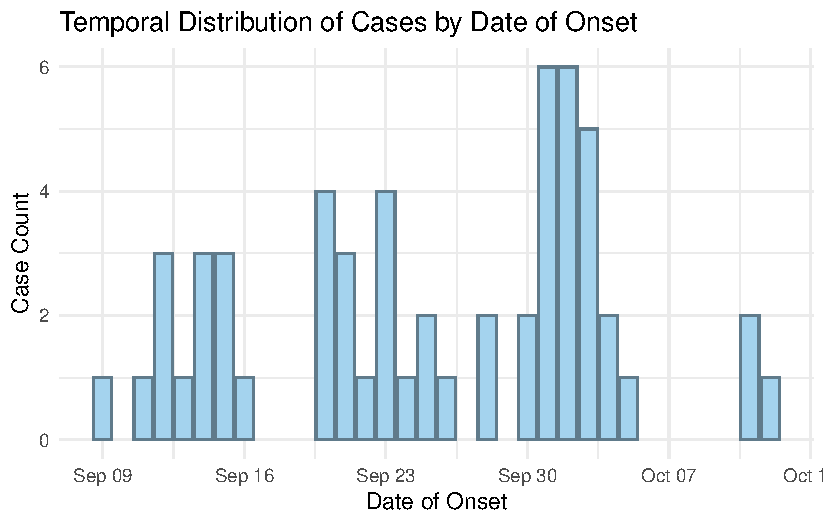
\includegraphics{Clean-Data-Work-in-Progress_files/figure-pdf/unnamed-chunk-7-1.pdf}

\begin{Shaded}
\begin{Highlighting}[]
\NormalTok{sdate }\OtherTok{\textless{}{-}} \FunctionTok{as.Date}\NormalTok{(}\FunctionTok{min}\NormalTok{(rff\_2024}\SpecialCharTok{$}\NormalTok{Date\_of\_Onset, }\AttributeTok{na.rm =} \ConstantTok{TRUE}\NormalTok{))}
\NormalTok{edate }\OtherTok{\textless{}{-}} \FunctionTok{as.Date}\NormalTok{(}\FunctionTok{max}\NormalTok{(rff\_2024}\SpecialCharTok{$}\NormalTok{Date\_of\_Onset, }\AttributeTok{na.rm =} \ConstantTok{TRUE}\NormalTok{))}

\NormalTok{sequeniald }\OtherTok{\textless{}{-}} \FunctionTok{seq.Date}\NormalTok{(sdate, edate, }\AttributeTok{by =} \StringTok{"day"}\NormalTok{)}

\NormalTok{numb\_suceptible }\OtherTok{\textless{}{-}} \FunctionTok{integer}\NormalTok{(}\AttributeTok{length =} \FunctionTok{length}\NormalTok{(sequeniald))}
\NormalTok{numb\_infectious }\OtherTok{\textless{}{-}} \FunctionTok{integer}\NormalTok{(}\AttributeTok{length =} \FunctionTok{length}\NormalTok{(sequeniald))}
\NormalTok{numb\_recovered }\OtherTok{\textless{}{-}} \FunctionTok{integer}\NormalTok{(}\AttributeTok{length =} \FunctionTok{length}\NormalTok{(sequeniald))}

\NormalTok{total\_pop }\OtherTok{\textless{}{-}} \FunctionTok{nrow}\NormalTok{(rff\_2024)}

\ControlFlowTok{for}\NormalTok{ (i }\ControlFlowTok{in} \FunctionTok{seq\_along}\NormalTok{(sequeniald)) \{}
\NormalTok{  current\_date }\OtherTok{\textless{}{-}}\NormalTok{ sequeniald[i]}
  
 
\NormalTok{  numb\_infectious[i] }\OtherTok{\textless{}{-}} \FunctionTok{sum}\NormalTok{(rff\_2024}\SpecialCharTok{$}\NormalTok{Date\_of\_Onset }\SpecialCharTok{\textless{}=}\NormalTok{ current\_date }\SpecialCharTok{\&} 
\NormalTok{                            (}\FunctionTok{is.na}\NormalTok{(rff\_2024}\SpecialCharTok{$}\NormalTok{Date\_of\_Recovery) }\SpecialCharTok{|}\NormalTok{ rff\_2024}\SpecialCharTok{$}\NormalTok{Date\_of\_Recovery }\SpecialCharTok{\textgreater{}}\NormalTok{ current\_date), }\AttributeTok{na.rm =} \ConstantTok{TRUE}\NormalTok{)}
  
\NormalTok{  numb\_recovered[i] }\OtherTok{\textless{}{-}} \FunctionTok{sum}\NormalTok{(rff\_2024}\SpecialCharTok{$}\NormalTok{Date\_of\_Recovery }\SpecialCharTok{\textless{}=}\NormalTok{ current\_date, }\AttributeTok{na.rm =} \ConstantTok{TRUE}\NormalTok{)}
  
\NormalTok{  numb\_suceptible[i] }\OtherTok{\textless{}{-}}\NormalTok{ total\_pop }\SpecialCharTok{{-}}\NormalTok{ numb\_infectious[i] }\SpecialCharTok{{-}}\NormalTok{ numb\_recovered[i]}
\NormalTok{\}}

\NormalTok{state\_no }\OtherTok{\textless{}{-}} \FunctionTok{data.frame}\NormalTok{(}
  \AttributeTok{Date =}\NormalTok{ sequeniald,}
  \AttributeTok{Susceptible =}\NormalTok{ numb\_suceptible,}
  \AttributeTok{Infectious =}\NormalTok{ numb\_infectious,}
  \AttributeTok{Recovered =}\NormalTok{ numb\_recovered}
\NormalTok{)}

\NormalTok{state\_no\_long }\OtherTok{\textless{}{-}} \FunctionTok{data.frame}\NormalTok{(}
  \AttributeTok{Date =} \FunctionTok{rep}\NormalTok{(sequeniald, }\AttributeTok{times =} \DecValTok{3}\NormalTok{),}
  \AttributeTok{State =} \FunctionTok{rep}\NormalTok{(}\FunctionTok{c}\NormalTok{(}\StringTok{"Susceptible"}\NormalTok{, }\StringTok{"Infectious"}\NormalTok{, }\StringTok{"Recovered"}\NormalTok{), }\AttributeTok{each =} \FunctionTok{length}\NormalTok{(sequeniald)),}
  \AttributeTok{Count =} \FunctionTok{c}\NormalTok{(numb\_suceptible, numb\_infectious, numb\_recovered)}
\NormalTok{)}

\FunctionTok{library}\NormalTok{(ggplot2)}
\FunctionTok{ggplot}\NormalTok{(state\_no\_long, }\FunctionTok{aes}\NormalTok{(}\AttributeTok{x =}\NormalTok{ Date, }\AttributeTok{y =}\NormalTok{ Count, }\AttributeTok{color =}\NormalTok{ State, }\AttributeTok{group =}\NormalTok{ State)) }\SpecialCharTok{+}
  \FunctionTok{geom\_line}\NormalTok{(}\AttributeTok{linewidth =} \DecValTok{1}\NormalTok{) }\SpecialCharTok{+}
  \FunctionTok{labs}\NormalTok{(}
    \AttributeTok{title =} \StringTok{"Number of Susceptible, Infectious, and Recovered Individuals by Day"}\NormalTok{,}
    \AttributeTok{x =} \StringTok{"Date"}\NormalTok{, }\AttributeTok{y =} \StringTok{"Count of individuals "}
\NormalTok{  ) }\SpecialCharTok{+}
  \FunctionTok{scale\_color\_manual}\NormalTok{(}
    \AttributeTok{values =} \FunctionTok{c}\NormalTok{(}\StringTok{"Susceptible"} \OtherTok{=} \StringTok{"chocolate3"}\NormalTok{, }\StringTok{"Infectious"} \OtherTok{=} \StringTok{"darkslategray"}\NormalTok{, }\StringTok{"Recovered"} \OtherTok{=} \StringTok{"goldenrod"}\NormalTok{)}
\NormalTok{  ) }\SpecialCharTok{+}
  \FunctionTok{scale\_x\_date}\NormalTok{(}
    \AttributeTok{breaks =}\NormalTok{ scales}\SpecialCharTok{::}\FunctionTok{date\_breaks}\NormalTok{(}\StringTok{"3 days"}\NormalTok{),}
    \AttributeTok{labels =}\NormalTok{ scales}\SpecialCharTok{::}\FunctionTok{date\_format}\NormalTok{(}\StringTok{"\%b \%d"}\NormalTok{)}
\NormalTok{  ) }\SpecialCharTok{+}
  \FunctionTok{theme\_minimal}\NormalTok{() }\SpecialCharTok{+}
  \FunctionTok{theme}\NormalTok{(}
    \AttributeTok{legend.title =} \FunctionTok{element\_blank}\NormalTok{(),}
    \AttributeTok{axis.text.x =} \FunctionTok{element\_text}\NormalTok{(}\AttributeTok{angle =} \DecValTok{45}\NormalTok{, }\AttributeTok{hjust =} \DecValTok{1}\NormalTok{)}
\NormalTok{  )}
\end{Highlighting}
\end{Shaded}

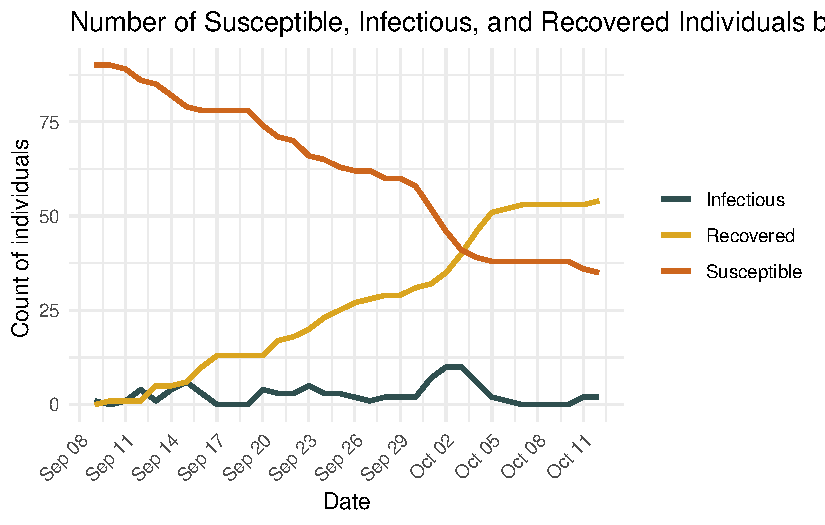
\includegraphics{Clean-Data-Work-in-Progress_files/figure-pdf/unnamed-chunk-8-1.pdf}

\begin{enumerate}
\def\labelenumi{\arabic{enumi}.}
\setcounter{enumi}{2}
\item
  Assign roles to outbreak team members

  Maria Paula - 1. Draw an epi curve (lecture week 4) -- required Mia -
  2. Natural history parameters (lecture week 1) -- required Aidan - 3.
  Reproduction numbers -- required Ravi - 4. Generate a mathematical
  model to answer a question -- required Maria Paula - 7. Herd immunity
  threshold
\item
  Begin brainstorming questions you have about the outbreak and plan to
  address

  \begin{enumerate}
  \def\labelenumii{\arabic{enumii}.}
  \item
    When was the peak of the outbreak and why did it peak there?
  \item
    What is the threshold of herd immunity?
  \item
    How infectious was the pathogen?
  \item
    Did transmission vary from course to course?
  \item
    Was there a difference in symptom onset for first years versus
    second years?
  \end{enumerate}
\end{enumerate}




\end{document}
